% This is part of Un soupçon de mathématique sans être agressif pour autant
% Copyright (c) 2015
%   Laurent Claessens
% See the file fdl-1.3.txt for copying conditions.

\begin{exercice}[\ldots\ldots/3]\label{exo2smath-0273}

    \begin{multicols}{2}

    \begin{center}
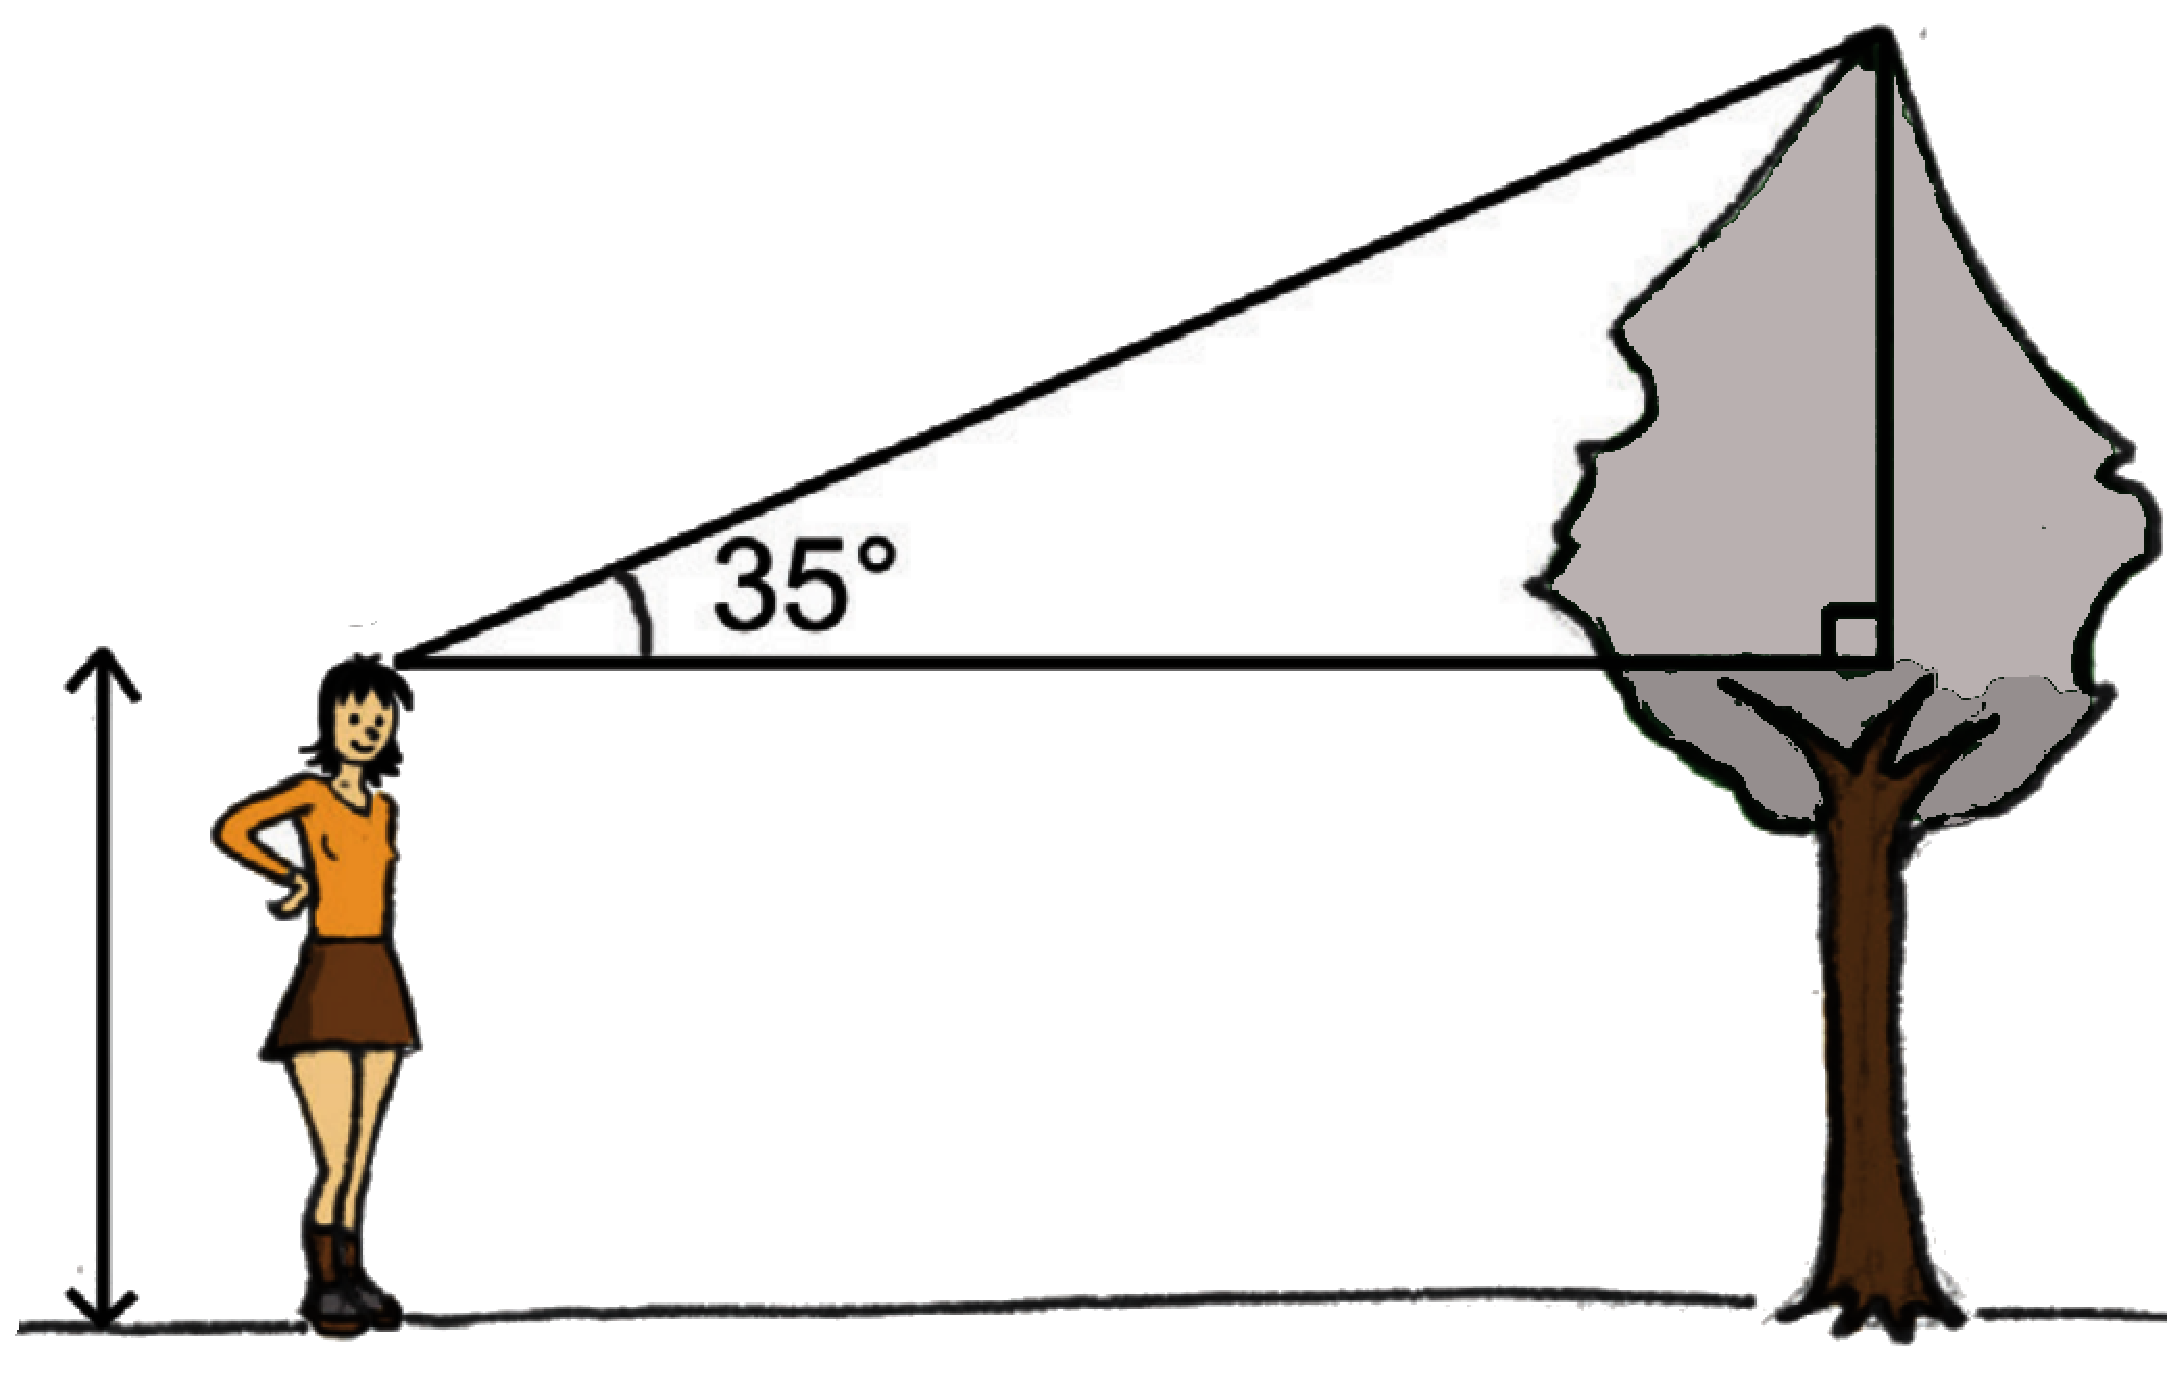
\includegraphics[width=5cm]{arbrecosinus2.pdf}
    \end{center}

    \columnbreak

    Sophie qui mesure \SI{1.75}{\meter} est à \SI{30}{\meter} d'un arbre. L'angle entre l'horizontale et le sommet de l'arbre est de \SI{35}{\degree}. Quelle est la hauteur de l'arbre ?

    \end{multicols}
\corrref{2smath-0273}
\end{exercice}
